

\newpage


%\paragraph{The PL--Norm Relation: Deriving a Special Case of Eqn.~(\ref{eqn:basic_relation}).}
\section{The PL--Norm Relation: Deriving a Special Case of Eqn.~(\ref{eqn:basic_relation})}
\label{sxn:appendix-derivation-pl-norm-relation}

Here, we derive Eqn.~(\ref{eqn:basic_relation}) in the special case of very small PL exponent, $\alpha \rightarrow 1$, for an $N \times M$ random matrix $\mathbf{W}$, {with $M=N, Q=1$, and with elements drawn from Eqn.~(\ref{eqn:ht_dstbn}).%
\footnote{We derive Eqn.~(\ref{eqn:basic_relation}) at what is sometimes pejoratively known as ``at a physics level of rigor.''  That is fine, as our justification will be seen in Section~\ref{sxn:emp}.  Recall our goal: to derive a very simple expression relating fitted PL exponents and Frobenius norms that usable by practical engineers working with state-of-the-art models, i.e., not simply small toy models.  There is very little ``rigorous'' work on HT-RMT, less still on understanding finite-sized effects of HT Universality.  Hopefully, our results will lead to more work along these lines.  }
That is, we establish this as an asymptotic relation for the VHT Universality class for very small exponents.

\michael{MM TO RECHECK DETAILS; and be careful below about $\mu$s and $\alpha$s.}
To start, recall that 
$$ 
\Vert \mathbf{W}\Vert_{F}^{2}=\mbox{Trace}[\mathbf{W}^{T}\mathbf{W}]=N\;\mbox{Trace}[\mathbf{X}]  .
$$
Since, for \nred{$\mu \gtrsim 0$}, \michael{NOT $\alpha$, but maybe 1?} 
the eigenvalue spectrum is dominated by a single large eigenvalue, it follows that
$$
\Vert \mathbf{W}\Vert_{F}^{2}\approx N\lambda^{max}  , 
$$
where $\lambda^{max}$ is the largest eigenvalue of the matrix $\mathbf{X}$ (with the $1/N$ normalization).
Taking the log of both sides of this expression and expanding leads to
%\begin{eqnarray*}
%\log\Vert \mathbf{W}\Vert_{F}^{2} 
%   &\approx& \log \left( N\lambda^{max} \right) \\
%   &=&       \log N+\log\lambda^{max}  .
%\end{eqnarray*}
\begin{eqnarray*}
\log\Vert \mathbf{W}\Vert_{F}^{2} 
   \approx \log \left( N\lambda^{max} \right) 
   =       \log N+\log\lambda^{max}  .
\end{eqnarray*}
Rearranging, we get that 
$$
\dfrac{\log\Vert \mathbf{W}\Vert_{F}^{2}}{\log\lambda^{max}}\approx \dfrac{\log N}{\log\lambda^{max}}+1  .
$$
Thus, for a parameter $\alpha$ satisfying Eqn.~(\ref{eqn:basic_relation}), we have that 
$$
\alpha\approx \dfrac{\log N}{\log\lambda^{max}}+1  .
$$
%%%
%%%$$
%%%\alpha-1\approx \dfrac{\log N}{\log\lambda^{max}}  .
%%%$$
%%%
Recall that the relation between $\alpha$ and $\mu$ for the VHT Universality class is given in Eqn.~(\ref{eqn:alpha_mu_vht}) as
$ %$$
\alpha=\frac{1}{2}\mu+1  .
$ %$$
Thus, to establish our result, we need to show that
$$
\dfrac{\log N}{\log\lambda^{max}}\approx\dfrac{1}{2}\mu  .
$$
To do this, we use the relation of Eqn.~(\ref{eqn:scaling_of_lambda_max}) for the tail statistic, i.e., that 
$ %$$
\lambda^{max}\approx N^{4/\mu-1}  .
$ %$$
Taking the log of both sides gives
$$
\log\lambda^{max}\approx\log N^{4/\mu-1}=(4/\mu-1)\log N  ,
$$
from which if follows that
$$
\dfrac{\log N}{\log\lambda^{max}}\approx\dfrac{\log N}{(4/\mu-1)\log N}=\dfrac{1}{4/\mu-1}   .
$$
Finally, we can form the Taylor Series for $\dfrac{1}{4/\mu-1}$ around $\mu=1.15\approx 1$, which gives 
$$
\dfrac{1}{4/\mu-1}\bigg\rvert_{\mu=1.15}\approx\dfrac{1}{2}\mu-\dfrac{1}{6}+\cdots\approx\dfrac{1}{2}\mu  .
$$
This established the approximate---and surprising---linear relation we want for $\mu \gtrsim 1$. 
%\michael{MM again, be careful below about $\mu$s and $\alpha$s.}



%\paragraph{The PL--Norm Relation: Finite-Size Effects.}
\section{The PL--Norm Relation: Finite-Size Effects.}
\label{sxn:appendix-finite-size}


Here, we consider finite-size effects in Eqn.~(\ref{eqn:basic_relation}), both within and across HT Universality classes, i.e., for both VHT and MHT matrices.
See Figure~\ref{fig:randW}, which  displays $\frac{\log\Vert\mathbf{W}\Vert^{2}_{F}}{\log\lambda^{max}}$ as a function of the fitted PL exponent $\alpha$, with varying sizes $N$ (with aspect ratio $Q=1$).
Recall that $\alpha \approx \frac{1}{2}\mu+1$ for finite-sized VHT random matrices, while $\alpha = a\mu+b$ for finite-sized MHT random matrices, where $a,b$ depend strongly on the size of the matrix.  Thus, $\mu\in(0,2)$ for VHT matrices corresponds to $\alpha\in(1,2)$, while $\alpha \approx(2,3)$ or $\alpha \approx(2,4)$ for MHT matrices.
%% $$
%% \dfrac{\log\Vert\mathbf{W}\Vert^{2}_{F}}{\log\lambda_{max}}\;\;vs.\;\;(\alpha)  .
%% $$
The numerical results in Figure~\ref{fig:randW} show that as $\alpha$ increases:
when $\alpha<2$, there exists a near-linear relation; and
when $\alpha>2$, for $N,M$ large, the relation saturates, becoming constant, while for smaller $N,M$, there exists a near-linear relation, but with strong finite-size effects.
These numerical results demonstrate that $ \log\Vert\mathbf{W}\Vert^{2}_{F}\approx\alpha\log\lambda^{max} $ works very well for VHT random matrices, for $\alpha<2$, and that it works moderately well for MHT matrices and even some WHT matrices.
In particular, for MHT matrices, the finite-size regime in which it holds moderately well when $N,M\sim\mathcal{O}(100-1000)$, which is typical for modern DNNs. 

\begin{figure*}[!htb]
   \centering
   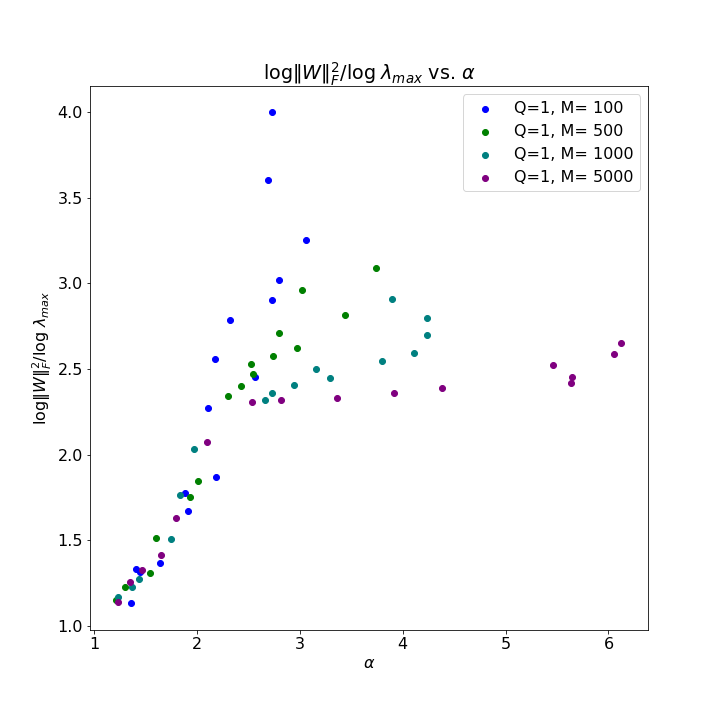
\includegraphics[scale=0.30]{img/Alpha-LogNorm-Relations.png}
   \caption{
            Numerical test of Eqn.~(\ref{eqn:basic_relation}) for random HT matrices across different HT Universality classes.
            \michael{Charles, change $M$ to $N$ in caption.}
           }
   \label{fig:randW}
\end{figure*}


%% \michael{Make sure what I include in the above par is enough for what I need here.}
%% \michael{Here is the place to make explicit the connection between $\alpha$ and $\mu$, for finite $N$ and asymptotically, and to say Eqns.~(\ref{eqn:alpha_mu_vht_and_mht}) holds for both VHT and MHT, for realistic values of $N$.}

%To understand this relation better, and to sketch a proof,
%we will generate the data for a number of a Heavy-Tailed random matrices, 
%with different power law exponents $\mu$.
%Note that this linear relation holds over several log scales.  However,
%the relation does deviate from linearity at the smaller values of $\alpha\;\log_{10}\;\lambda_{max}$.
%This is readily explained below .  


%%MM%% This approximate relation formally only hold in the asymptotic limit of very small power law exponents $\alpha\rightarrow 1$ for
%%MM%% random heavy tailed matrices, but using Universality, we can safely extend it up to the finite-size MHT class, with
%%MM%% exponents $\alpha=4$ (and larger).  



%\paragraph{The PL--Norm Relation: Random Matrices versus Real Data.}
\section{The PL--Norm Relation: Random Matrices versus Real Data}
\label{sxn:appendix-random-vs-real}

\begin{figure*}[!htb]
    \centering
    \subfigure[Random Pareto Matrices] {
        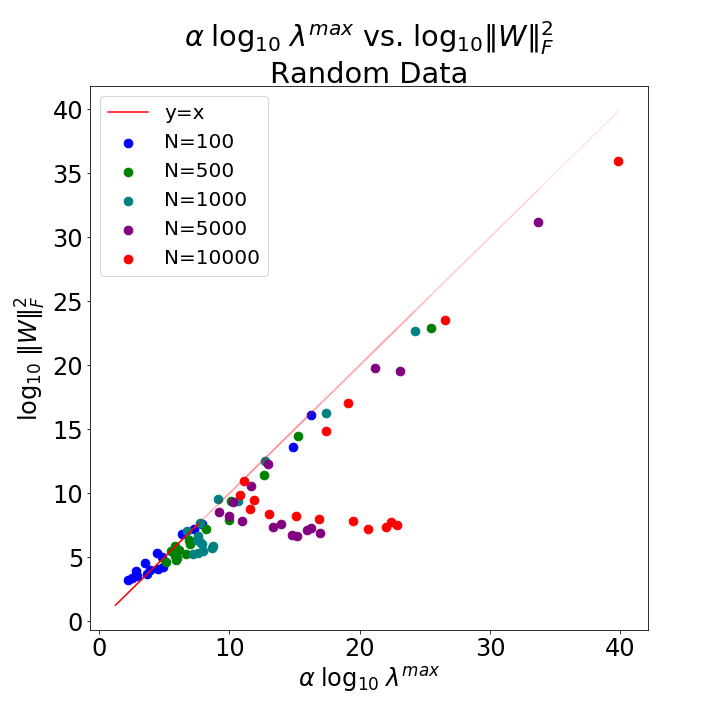
\includegraphics[scale=0.30]{img/relation-rand.png} 
        \label{fig:relation-rand}
    }
    \subfigure[VGG11 Weight matrices]{
        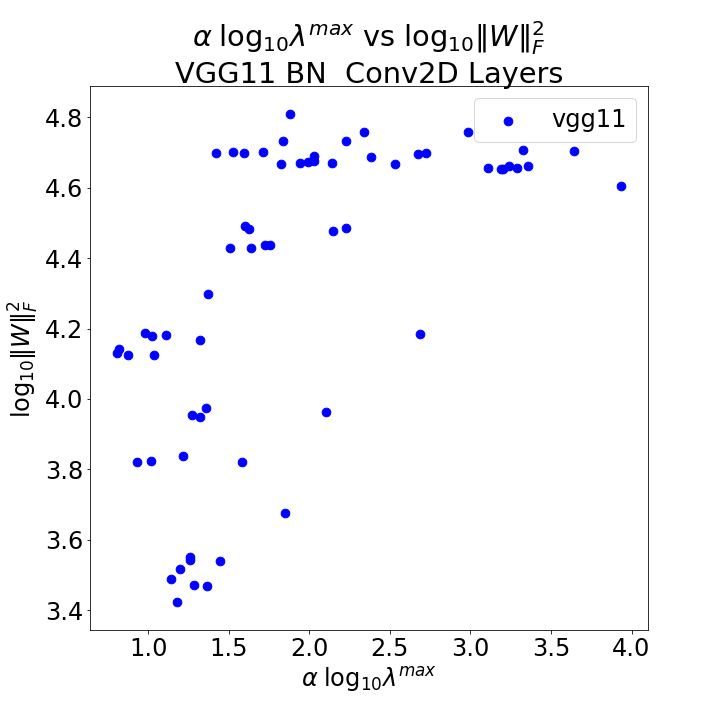
\includegraphics[scale=0.30]{img/relation-vgg11.png} 
        \label{fig:relation-vgg11}
    }
        \caption{Relation between $\alpha\log_{10}\lambda^{max}$ and $\log_{10}\Vert\mathbf{W}\Vert^{2}_{F}$ for random (Pareto) matrices and real (VGG11) DNN weight matrices.
                 \michael{Charles, change $M$ to $N$ in caption.}
                 }
    \label{fig:relations}
\end{figure*}

Here, we show numerically that the qualitative form of Eqn.~(\ref{eqn:basic_relation}) holds more generally than the special case derived previously, including into the MHT Universality class, for both random and real data.
To illustrate this, we generate a large number of HT random matrices $\mathbf{W}^{rand}(\mu)$, with varying sizes $N$ (with aspect ratio $Q=1$), drawn from a Pareto distribution of Eqn.~(\ref{eqn:ht_dstbn}), with exponents $\mu\in[0.5, 5]$.
We then fit the ESD of each $\mathbf{W}^{rand}(\mu)$ to a PL using the method of Clauset et al.~\cite{CSN09_powerlaw,ABP14} to obtain the empirical exponent $\alpha$.   
Figure~\ref{fig:relation-rand} shows that there is a near-perfect relation between $ \alpha\log\lambda^{max}$ and $\log\Vert\mathbf{W}\Vert^{2}_{F} $.
We also performed a similar PL fit for VGG11 weight matrices.
(See Section~\ref{sxn:emp} for some details on the VGG11 model.)
Figure~\ref{fig:relation-vgg11} shows the results, demonstrating an increasing relation until $ \alpha\log_{10}\lambda^{max} \approx 2.5$ and a saturation after that point.
Figure~\ref{fig:relations} illustrates
(among other things\footnote{Clearly, there are also differences between the HT random and the real DNN matrices, most notably that $ \alpha\log\lambda^{max} $ achieves much larger values for the random matrices.  This is discussed in more detail in Appendix~\ref{sxn:appendix-universality}.})
that multiplying $\alpha$ by $\log_{10}\lambda^{max}$ leads to a relation that increases linearly with the (log of the squared) Frobenius norm for HT random matrices, and that the two quantities are linearly correlated for real DNN weight matrices.

%% \michael{Maybe comment also about how points large on the X axis have smaller $\alpha$.}
%% 
%% \charlesX{LEAD INTO HOW WE GOT THIS SECTION... PRESENT THE PL-NORM RELATION, SHOW THAT IT IS THE RIGHT SLOPE, AND HOW THE FINITE SIZE  EFFECTS LET US EXTEND THIS RELATION ACROSS UNIVERSALITY CLASSES IN ROUGH WAY, GIVING A USEFUL METRIC FOR ENGINEERING WORK.  REAL DATA IS SHOWN.  HAS 4 PLOTS.  USES NUMERICAL METHODS DESCRIBED ABOVE.  WE MAY WANT PSEUDOCODE ALSO ?}



\section{Random Pareto versus Non-random DNN Matrices} 
%\section{Heavy-Tailed Universality: Random Pareto versus Non-random DNN Matrices} 
\label{sxn:appendix-universality}

When we use Universality, as we do in our derivation of the basic PL--Norm Relation, we would like a method that applies both to HT random matrices as well as to non-random, indeed strongly-correlated, pre-trained DNN layer weight matrices that (as evidenced by their ESD properties) are in a HT Universality class.  
To accomplish this, however, requires some care: while the pre-trained $\mathbf{W}$ matrices do have ESDs that display empirical signatures of HT Universality~\cite{MM18_TR}, they are \emph{not} random Pareto matrices.
Many of their properties, including their empirical Frobenius norms, behave very differently than that of a random Pareto matrix.  
(We saw this in Figure~\ref{fig:relations}, which showed that $ \alpha\log\lambda^{max} $ achieves much larger values for HT random matrices than real DNN weight matrices.)

To illustrate this, we generate a large number of HT random matrices $\mathbf{W}^{rand}(\mu)$, with exponents $\mu\in[0.5, 5]$, as described in Section~\ref{sxn:theory-new}.
%
We then fit the ESD of each $\mathbf{W}^{rand}(\mu)$ to a PL using the method of Clauset et al.~\cite{CSN09_powerlaw,ABP14} to obtain the empirical exponent $\alpha$. 
Figure~\ref{fig:fro-rand} displays the relationship between the (log of the squared) Frobenius norm and the $\mu$ exponents for these randomly-generated Pareto matrices.
(Similar but noisier plots would arise if we plotted as a function of $\alpha$, due to imperfections in the PL fit.)
We did the same for the weight matrices (extracted from the Conv2D Feature Maps) from the pre-trained VGG11 DNN, again as described in Section~\ref{sxn:theory-new}.
Figure~\ref{fig:fro-vgg11} displays these results, here as a function of $\alpha$.
\michael{Charles, maybe plot both as a function of $\alpha$, since they are different, and consistent with text.}

\begin{figure*}[!htb]
   \centering
   \subfigure[Random Pareto Matrices] {
      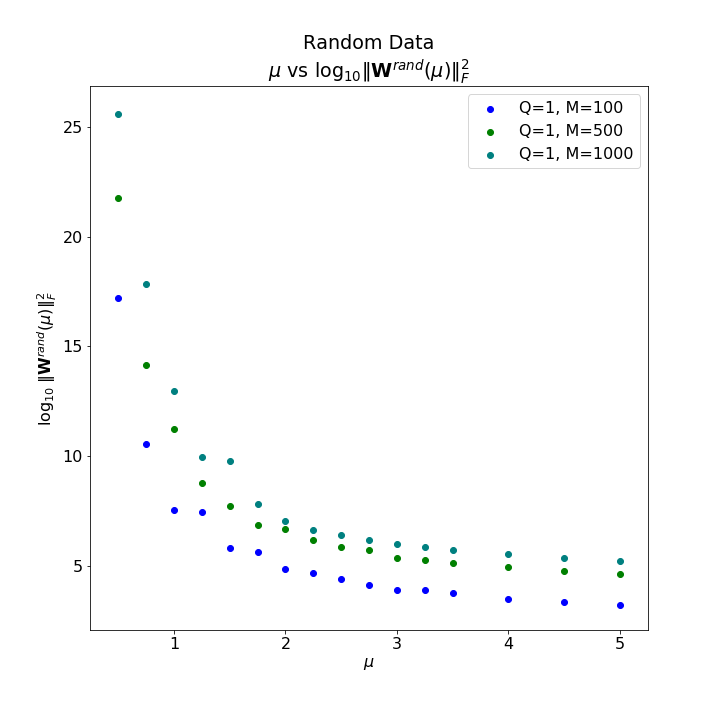
\includegraphics[scale=0.30]{img/fro-rand.png} 
      \label{fig:fro-rand}
   }
   \subfigure[Pre-trained VGG11 Weight Matrices]{
      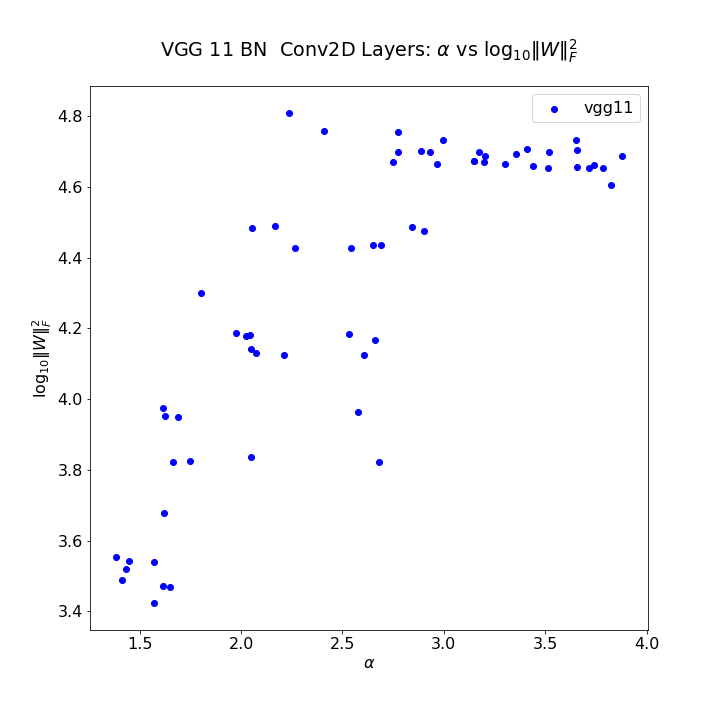
\includegraphics[scale=0.30]{img/fro-vgg11.png} 
      \label{fig:fro-vgg11}
   }
   \caption{Dependence of Frobenius norm on PL exponents for random Pareto versus pre-trained DNN matrices.  }
   \label{fig:fnorm}
\end{figure*}

The properties of $\Vert\mathbf{W}\Vert^{2}_{F}$ for the random Pareto versus real/ron-random DNN weight matrices are quite different.
For a random Pareto matrix, $\mathbf{W}^{rand}(\mu)$, the Frobenius norm $\Vert\mathbf{W}^{rand}(\mu)\Vert^{2}_{F}$ 
\emph{decreases with increasing exponent} $(\mu)$; and there is a modest finite-size effect.
(In addition, as the tails of the ESD $\rho(\lambda)$ get heavier, the largest eigenvalue $\lambda^{max}$ of $\mathbf{X}$ scales with the largest element of $\mathbf{W}^{rand}(\mu)$.) 
% \michael{$\alpha$ or $\mu$ here.}
% \michael{Cite something or show this.}
For the weight matrices of a pre-trained DNN, however, the Frobenius norm $\Vert\mathbf{W}\Vert^{2}_{F}$ \emph{increases with increasing exponent} $(\alpha)$, saturating at $\alpha\approx 3$.
This happens because, due to the training process, the $\mathbf{W}$ matrices themselves are highly-correlated, and not random matrices with a single large, atypical element.
In spite of this, the ESD $\rho(\lambda)$ of these pre-trained correlations matrices $\mathbf{X}$ display Universal HT behavior~\cite{MM18_TR}; and, as shown in Figure~\ref{fig:relation-vgg11}, 
Eqn.~(\ref{eqn:basic_relation}) is approximately satisfied, in the sense that 
$\alpha\log\lambda^{max}$ is positively correlated with $\log\Vert\mathbf{W}\Vert^{2}_{F} $.
This is one of the remarkable properties of Universality (and it shows why some care must be taken in applying these Universality principles).


\section{Additional Empirical Results}
\label{sxn:appendix-addl-empirical}

In addition to the VGG and ResNet series of models, we examined a wide range of other DNNs.
Here, we summarize some of those results.

\paragraph{More Pre-trained Models.}

Here are results for more pre-trained models.
See
Table~\ref{table:models_more}
as well as 
Figure~\ref{fig:models_more} 
for details.
XXX.  SOME COMMENTS.

\begin{table}[!htb]
\small
\begin{center}
\begin{tabular}{|p{1in}|c|c|c|c|c|c|c|}
\hline
Architecture 
 & Model
 & Test Accuracy \\
\hline
GoogLeNet & & \\
\hline
ResNeXt & & \\
\hline
SqueezeNet & & \\
\hline
\end{tabular}
\end{center}
\caption{Results for more models.
         \michael{Charles, why is this split off from the next table.}
        }
\label{table:models_more}
\end{table}

\begin{figure*}[!htb]
   \centering
   \subfigure[DenseNet] {
       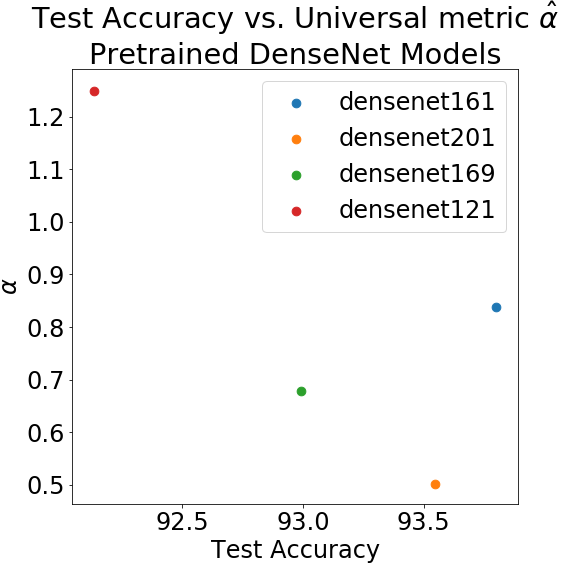
\includegraphics[scale=0.30]{img/densenet-pytorch-w_alphas.png} 
       \label{fig:densenet}
   }
   \subfigure[SqueezeNet]{
       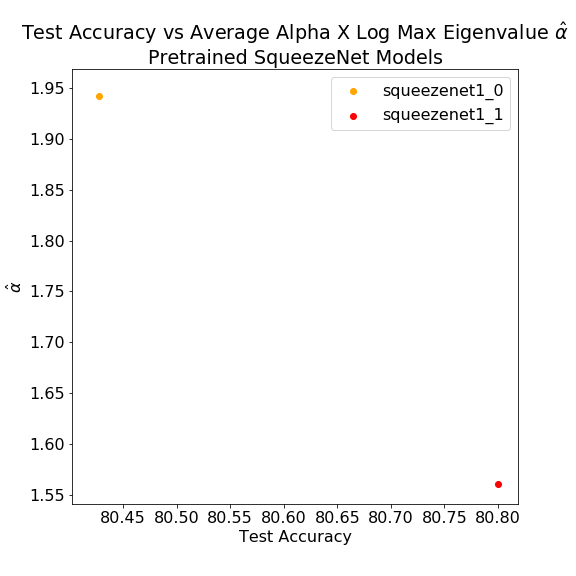
\includegraphics[scale=0.30]{img/squeezenet-pytorch-w_alphas.png} 
       \label{fig:squeezenet}
   }
   \caption{
      Pre-trained 
      Densenet and SqueezeNet PyTorch 
      Models.
      Test Accuracy versus
      $\hat{\alpha}$.
      \michael{Charles, fix to be consistent with other figures.}
           }
   \label{fig:models_more}
\end{figure*}


\paragraph{Still More Pre-trained Models.}

Here are results for still more pre-trained models.
See
Table~\ref{table:models_still_more}
as well as
Figures~\ref{fig:still_more_1} and \ref{fig:still_more_2}
for details.
XXX.  SOME COMMENTS.


\begin{table}[!htb]
\small
\begin{center}
\begin{tabular}{|p{1in}|c|c|c|c|c|c|c|}
\hline
Architecture 
 & Model
 & Top 1 Error \\
 \hline
 DenseNet & densenet121 & 25.57 & \\
& densenet161 & 22.86 & \\
& densenet169 & 24.4 & \\
& densenet201 & 23.1 & \\\hline
DPN & dpn68 & 24.17 & \\
& dpn98 & 20.81 & \\
& dpn131 & 20.54 & \\
\hline
MeNet & menet108\_8x1\_g3 & 43.92 & \\
& menet128\_8x1\_g4 & 43.95 & \\
& menet228\_12x1\_g3 & 33.57 & \\
& menet256\_12x1\_g4 & 33.41 & \\
& menet348\_12x1\_g3 & 30.1 & \\
& menet352\_12x1\_g8 & 33.31 & \\
& menet456\_24x1\_g3 & 28.4 & \\
\hline
MobileNet & mobilenet\_wd4 & 46.26 & \\
& mobilenet\_wd2 & 36.3 & \\
& mobilenet\_w3d4 & 33.54 & \\
& mobilenet\_w1 & 29.86 & \\
\hline
MobileNetV2 & mobilenetv2\_wd4 & 49.72 & \\
& mobilenetv2\_wd2 & 36.54 & \\
& mobilenetv2\_w3d4 & 31.89 & \\
& mobilenetv2\_w1 & 29.31 & \\
\hline
FDMobileNet & fdmobilenet\_wd4 & 55.77 & \\
& fdmobilenet\_wd2 & 43.85 & \\
& fdmobilenet\_w1 & 34.7 & \\
\hline
SE-ResNet & seresnet50 & 22.47 & \\
& seresnet101 & 21.88 & \\
& seresnet152 & 21.48 & \\
\hline
SE-ResNeXt & seresnext50\_32x4d & 21.0 & \\
& seresnext101\_32x4d & 19.96 & \\
\hline
ShuffleNet & shufflenetv2\_wd2 & 41.48 & \\
& shufflenetv2\_w1 & 34.39 & \\
\hline
\end{tabular}
\end{center}
\caption{Results for still more models.
         \michael{Charles, why is this split off from previous table.}
         \michael{Charles, why is CondenseNet missing.}
         \michael{Charles, why Test Accuracy for others and Top 1 Error here.}
        }
\label{table:models_still_more}
\end{table}


\begin{figure*}[!htb]
   \centering
   \subfigure[CondenseNet]{
       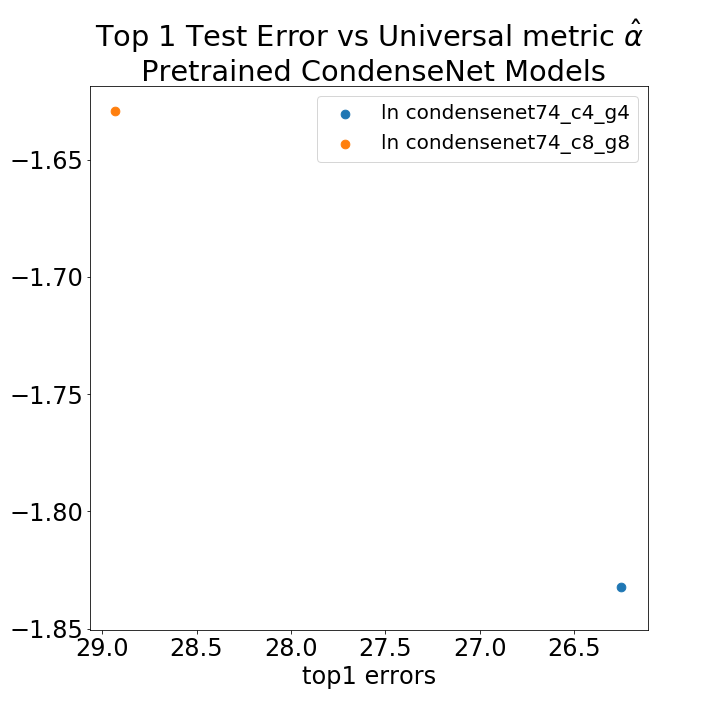
\includegraphics[scale=0.19]{img/CondenseNet-w_alphas.png} 
       \label{fig:densenet-small}
   }
   \subfigure[DPN]{
       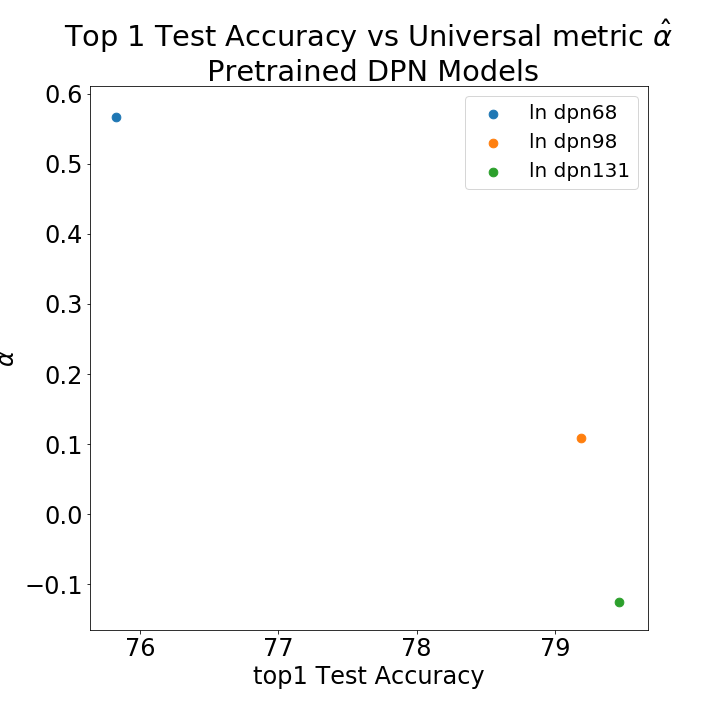
\includegraphics[scale=0.19]{img/DPN-w_alphas.png} 
       \label{fig:dpn-net}
   }
   \subfigure[ShuffleNet]{
      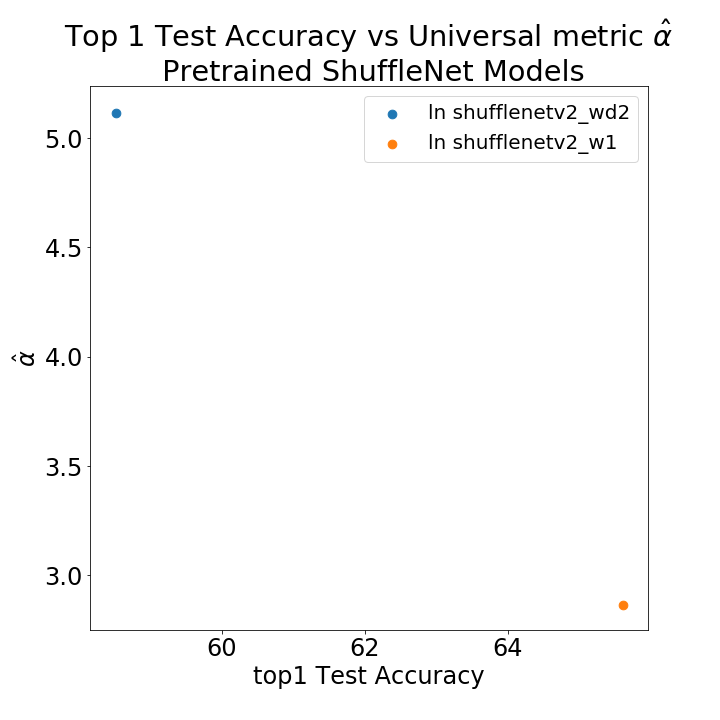
\includegraphics[scale=0.19]{img/ShuffleNet-w_alphas.png}
      \label{fig:shufflenet-small}
   }
   \caption{
      Pre-trained 
      CondenseNet, DPN, and ShuffleNet
      Models.
      Top 1 Test error versus
      $\hat{\alpha}$.
      \michael{Charles, fix to be consistent with other figures.}
           }
   \label{fig:still_more_1}
\end{figure*}


\begin{figure*}[!htb]
   \centering
   \subfigure[MobileNet]{
      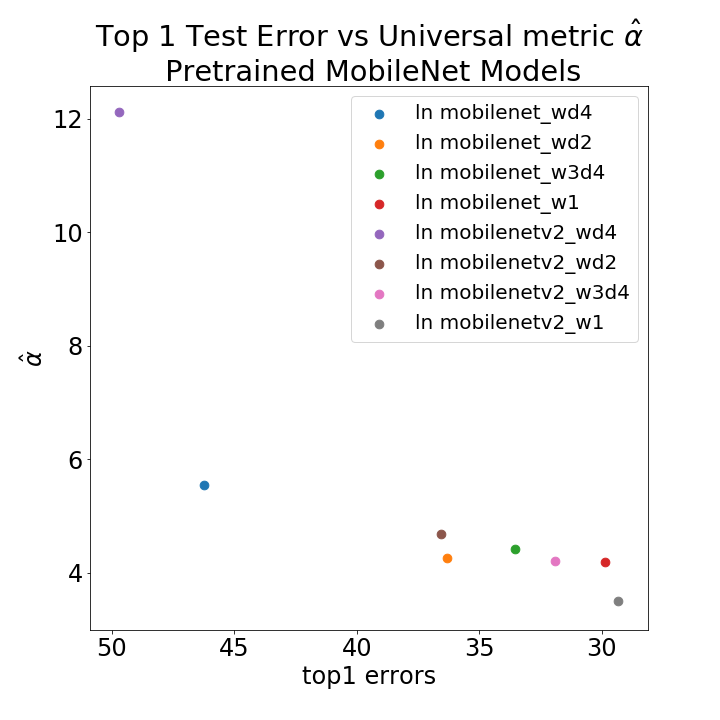
\includegraphics[scale=0.19]{img/MobileNet-w_alphas.png} 
      \label{fig:resnet-small}
   }
   \subfigure[SeResNet]{
      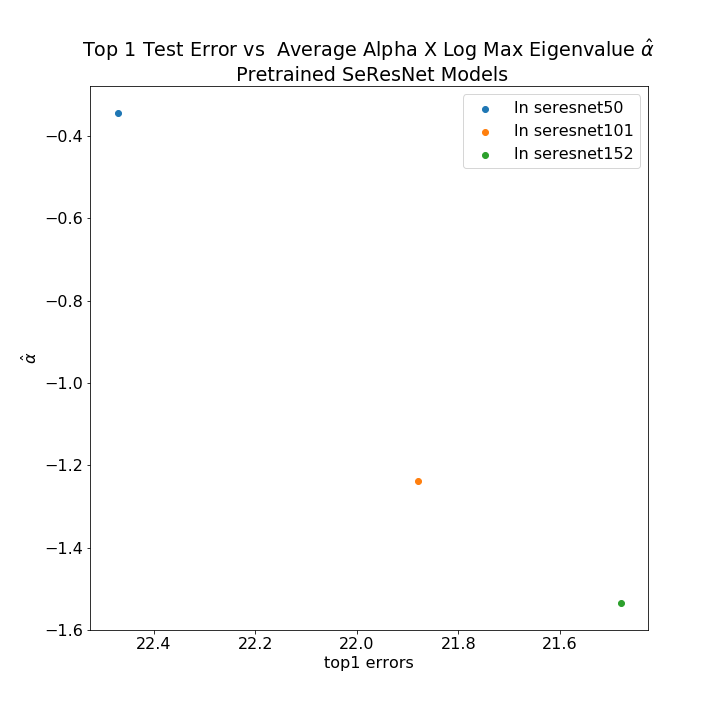
\includegraphics[scale=0.19]{img/SeResNet-w_alphas.png}
      \label{fig:shufflenet-small}
   }
   \subfigure[SeResNeXt]{
      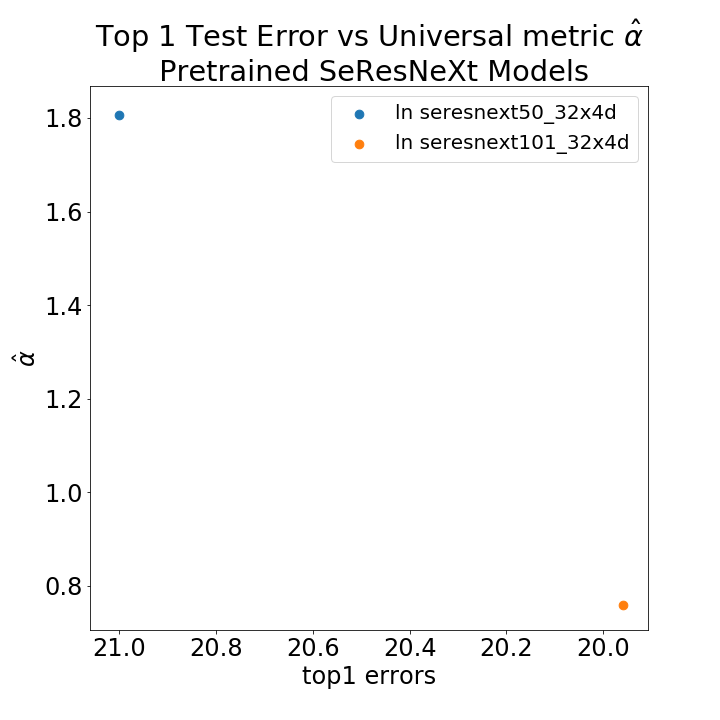
\includegraphics[scale=0.19]{img/SeResNeXt-w_alphas.png}
      \label{fig:shufflenet-small}
   }
   \caption{
      Pre-trained 
      MeNet, SeResNet, and SeResNeXt
      Models.
      Top 1 Test error versus
      $\hat{\alpha}$.
      \michael{Charles, fix to be consistent with other figures.}
           }
   \label{fig:still_more_2}
\end{figure*}


\paragraph{Counterexamples.}
There are of course exceptions here and there.
See
Figure~\ref{fig:counter-examples}
as well as 
Table~\ref{table:models_still_more}
for details on the counterexamples.
XXX.  COMMENTS.

\begin{figure*}[!htb]
   \centering
   \subfigure[ResNeXt]{
      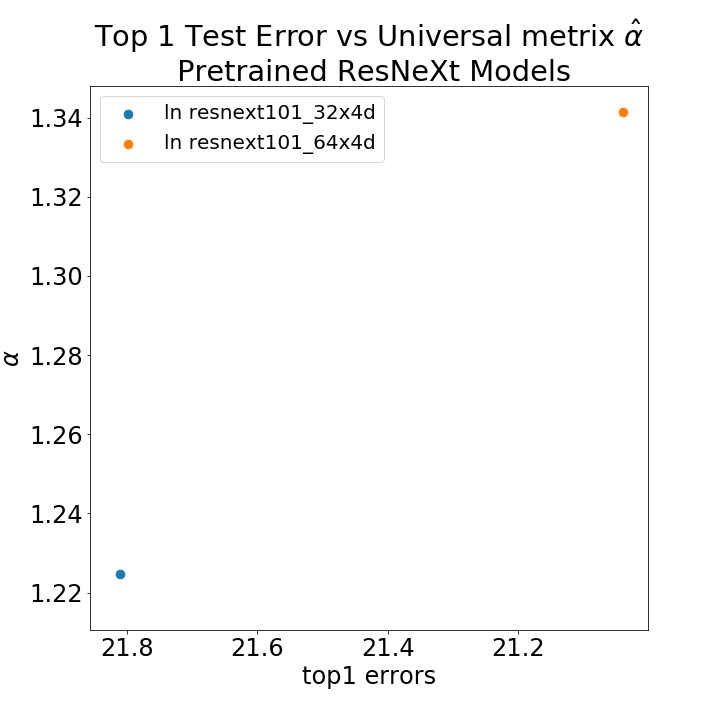
\includegraphics[scale=0.19]{img/ResNeXt-w_alphas.png} 
      \label{fig:resnet-small}
   }
   \subfigure[MeNet]{
      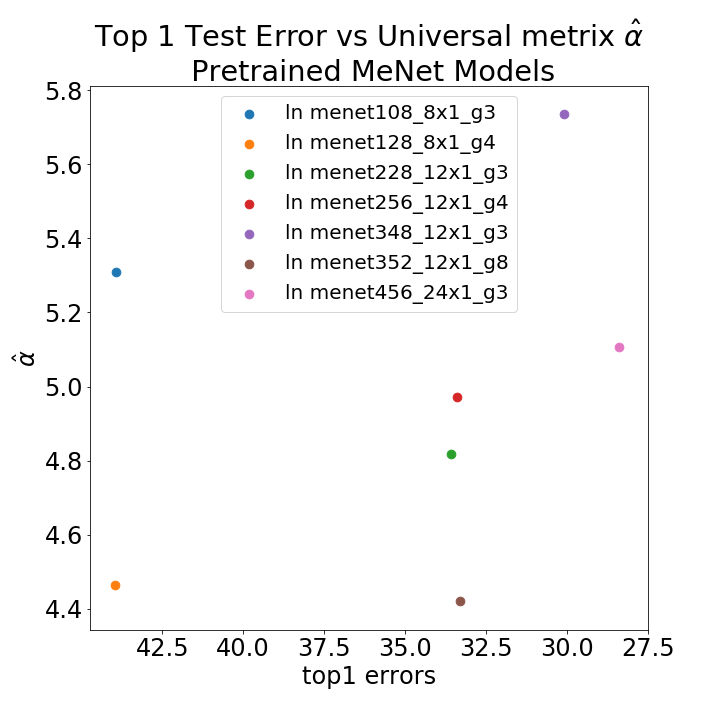
\includegraphics[scale=0.19]{img/MeNet-w_alphas.png} 
      \label{fig:menet-net}
   }
   \subfigure[FDMobileNet]{
      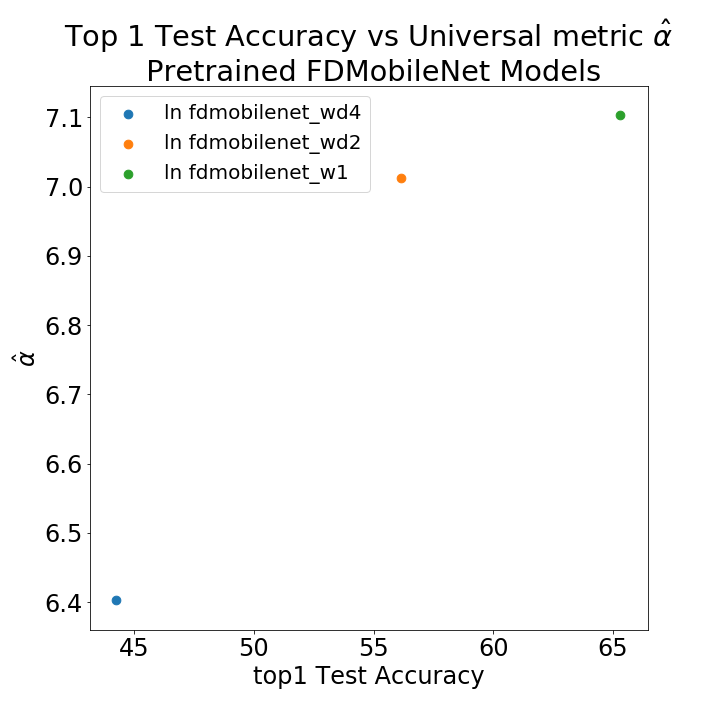
\includegraphics[scale=0.19]{img/FDMobileNet-w_alphas.png} 
      \label{fig:resnet-small}
   }
   \caption{
      Pre-trained 
      ResNeXt, MeNet, and FDMobileNet
      Models 
      that provide counterexamples to our main trends.
      Top 1 Test error versus
      $\hat{\alpha}$.
      \michael{Charles, fix to be consistent with other figures.}
           }
   \label{fig:counter-examples}
\end{figure*}





\section{Additional Discussion}
\label{sxn:appendix-addl-discussion}

We have presented an \emph{unsupervised} capacity control metric which predicts trends in test accuracies of a trained DNN---without peeking at the test data. 
This complexity metic, $\hat{\alpha}$ of Eqn.~(\ref{eqn:alpha_hat_specific}), is a weighted average of the PL exponents $\alpha$ for each layer weight matrix, where $\alpha$ is defined in the recent HT-SR Theory~\cite{MM17_TR,MM18_TR}, and where the weights are the largest eigenvalue $\lambda^{max}$ of the correlation matrix $\mathbf{X}$.  
%
We examine several commonly-available, pre-trained, production-quality DNNs by plotting $\hat{\alpha}$ versus the reported test accuracies.
This covers classes of DNN architectures including the VGG models, ResNet, DenseNet, etc. 
In nearly every class, and except for a few counterexamples, smaller $\hat{\alpha}$ corresponds to better average test accuracies, thereby providing a strong predictor of model quality.
%
We also show that this new complexity metric $\hat{\alpha}$ is approximately the average log of the Frobenius norm of the layer weight matrices, $\langle\log\Vert\mathbf{W}\Vert_{F}^{2}\rangle$, when accounting for finite-size effects.
This provides an interesting connection between the Statistical Physics approach to learning (from Martin and Mahoney~\cite{MM17_TR,MM18_TR}, that we extend here) and methods such as that of Liao et al.~\cite{LMBx18_TR}, who use norm-based capacity control metrics to bound worst-case generalization~error.

We should mention two higher-level comments.
%
First, 
one of the main insights of our approach is to highlight the importance of what might seem to be a technical issue to ignore, but which in our experience is \emph{extremely} important: the scaling or normalization for weight matrices used in the DNN, and how this relates to the difference between finite-size versus asymptotic effects.
\michael{Modify slightly since we don't go into as much detail about our scaling problems, so modify these comments.}
This scaling issue has been highlighted perhaps most recently by Bartlett et al.~\cite{BFT17_TR} and Liao et al.~\cite{LMBx18_TR}.
The latter were interested in showing that classical generalization bounds can be tight---when normalization is performed appropriately.
Our approach complements theirs; but, to our knowledge, our approach is the first to highlight the connection with finite-size effects.
%
Second, 
%it is worth emphasizing that 
we are taking a 
very %somewhat 
non-standard approach (at least for the DNN and ML communities) to address our main question.
We didn't train/retrain lots and lots of (typically rather small) models, analyzing training/test curves, trying to glean from them bits of insight that might then extrapolate to more realistic models.
Instead, we took advantage of the fact that there already exist many (typically rather large) publicly-available pre-trained models, and we analyzed the properties of these models.
That is, we viewed these publicly-available pre-trained models as artifacts of the world that achieve state-of-the-art performance in computer vision, NLP, and related applications; and we attempted to understand why.
To do so, we analyzed the empirical (spectral) properties of these models; 
%from this, we formed a hypothesis as to why they perform well; 
and we then extracted data-dependent metrics to predict their generalization performance on production-quality models.
Given well-known challenges associated with training, 
%and given our results here as well as other recent results~\cite{MM18_TR},
we suggest that this methodology be applied more generally.

Finally, one interesting aspect of our approach is that we can apply these complexity metrics \emph{across related DNN architectures}. 
This is in contrast to the standard practice in ML.
The equivalent notion would be to compare margins across SVMs, applied to the same data, but with different kernels. 
One loose interpretation is that a set of related of DNN models (i.e., VGG11, VGG13, etc.) is analogous to a single, very complicated kernel, and that the hierarchy of architectures is analogous to the hierarchy of hypothesis spaces in more traditional VC theory.
%\charlesX{more here ?  like this ?}
%\michael{Let's discuss this, to see what we can squeeze, given what is now popular.}   

We expect our result will have applications in the fine-tuning of pre-trained DNNs used for transfer learning, as in NLP and related applications.
Moreover, because we do not need to peek at the test data, our approach may prevent information from leaking from the test set into the model, thereby helping to prevent overtraining and making fined-tuned DNNs more robust.
Finally, our work also leads to a much harder theoretical question: is it possible to characterize properties of realistic DNNs to determine whether a DNN is overtrained---without peeking at the test data?  
 

{ \iffalse

\newpage
\section{Appendix: Derivation of two relations}
\label{sxn:appendix-derivation-two-relations}

Here we derive the two relations, Eqns.~(\ref{eqn:alpha_mu_vht_and_mht}) and~(\ref{eqn:scaling_of_lambda_max}).
\michael{Maybe do this later.}

\fi }


{ \iffalse 

\newpage
\section{Appendix: Michael's Longer Derivation}
\label{sxn:appendix-michael_derivation}

\michael{MM probably remove this entirely, unless relate to synthetic empirical results.}

Here, we derive an expression for the ratio of the log of the Frobenius norm of $W$ to the log of the spectral norm of $W$.
Once we settle on presentation, with normaliation, etc., this will probably be a ``subroutine'' in our analysis.
To simplify things, we will be interested in the matrix $W$, and in particular the Frobenius norm $\|W\|_F$ and spectral norm $\|W\|_2$ of this matrix.
Then, given these expressions, we will derive other things, e.g., norms of correlation matrices with different normalizations, etc., by using different normalizations.  

Recall that we are modeling the matrix $W$ as a random matrix with heavy-tailed entries.
XXX.  WE MIGHT WANT A FIGURE SHOWING THE REAL DATA LOOKS LIKE THIS, LIKE THE BURDA PAPER.
Thus, the Frobenius norm is going to be related to the second moment of the entries, and the spectral norm is going to be related to the largest entry.
XXX.  CITE AUFFINGER PAPER FOR EXACTLY THE RANGE OF VALIDITY OF THIS.
An important issue will be the power law exponent, since---depending on it---familiar results will hold or will fail to hold.
For the moment, let's ignore that we are dealing with matrices, and let's focus on drawing elements from a heavy-tailed distribution, and computing various moments and extreme values of empirical draws.

Consider the extreme case of a HT distribution, namely a PL distribution.
XXX.  INCLUDE SOMETHING ABOUT SLOWLY VARYING FUNCTION AS WELL AS XMIN VALUE.
Up to a slowly-varying function, the general form of the probability distribution function is
$$
p(x) = \frac{C}{x^{1+\mu}}  = C x^{-1-\mu} , 
$$
where $\mu > -1$, and where $x \in [x_{min},\infty)$.
The cdf 
XXX ACTUALLY ONE MINUS THAT 
is then
$$
P_{\ge}(x) = \int_x^{\infty} p(x^{\prime}) dx^{\prime} 
           = \frac{C}{\mu} \frac{1}{x^{\mu}}  
           = \frac{C}{\mu} x^{-\mu}  .
$$
In order to compute $C$ and normalize these expressions, let
\begin{eqnarray*}
1 = \int_{x_{min}}^{\infty} p(x) dx 
  = C \int_{x_{min}}^{\infty} x^{-1-\mu} dx 
  = \frac{C}{-\mu} x^{-\mu} |_{x_{min}}^{\infty}  
  = \frac{C}{\mu} x_{min}^{-\mu}   ,
\end{eqnarray*}
which is valid (i.e., the integral converges and exists) if $\mu > 0$.
From this, is follows that the normalization constant is
\begin{equation}
C = \mu x_{min}^{\mu}  .
\label{eqn:pl_normalization}
\end{equation}
Thus, if $\mu > 0$, then the probability distribution function is 
\begin{equation}
p(x) 
%     = \frac{\mu}{x_{min}}\left( \frac{x_{min}}{x}\right)^{1+\mu}  
     = \frac{\mu}{x_{min}}\left( \frac{x}{x_{min}}\right)^{-1-\mu}  ,
\label{eqn:pl_pdf}
\end{equation}
and the cdf 
XXX ACTUALLY ONE MINUS THAT
is 
\begin{equation}
P_{\ge}(x) 
%           = \left( \frac{x_{min}}{x} \right)^{\mu}  
           = \left( \frac{x}{x_{min}} \right)^{-\mu}  .
\label{eqn:pl_one_minus_cdf}
\end{equation}
XXX.  MENTION SLOWLY VARYING THING, MAYBE AS CLAUSET DID.

An important aspect of heavy-tailed probability distributions is that extreme values, i.e., values very far from the mean (when the mean is even defined) are not extremely uncommon (as they are for distributions in the Gaussian universality class).
Of particular relevance for us is the largest value $x_{max}$ obtained when sampling from Eqn.~(\ref{eqn:pl_pdf}) in $n$ i.i.d. trials.
It is known, see e.g.~\cite{SornetteBook,BouchaudPotters03,newman2005_zipf}, that the expectation of $x_{max}$ for $\mu\in(1,2)$ 
XXX IS THIS TRUE FOR MORE GENERAL PL PARAMETERS
is given~by:
$$
\ExpectBracket{x_{max}} \approx x_{min} n^{1/\mu}  .
$$

Let's return to the expression given in Eqn.~(\ref{eqn:pl_pdf}) and compute the first few moments of this distribution.
The first moment is
\begin{eqnarray*}
\ExpectBracket{x} = \int_{x_{min}}^{\infty} x p(x) dx  
                  = C \int_{x_{min}}^{\infty} x^{-\mu} dx 
                  = \frac{C}{1-\mu} x^{1-\mu} |_{x_{min}}^{\infty} 
                  = \frac{\mu}{\mu-1} x_{min}    ,
\end{eqnarray*}
which is valid if $\mu > 1$.
Similarly, the second moment is
\begin{eqnarray*}
\ExpectBracket{x^2} = \int_{x_{min}}^{\infty} x^2 p(x) dx  
                    = C \int_{x_{min}}^{\infty} x^{1-\mu} dx 
                    = \frac{C}{2-\mu} x^{2-\mu} |_{x_{min}}^{\infty} 
                    = \frac{\mu}{\mu-2} x_{min}^2  ,  
\end{eqnarray*}
which is valid if $\mu > 2$.
While this second moment expression is valid for $\mu > 2$, we are going to want a similar expression for $\mu \in (1,2)$.
For this we can integrate up to $x_{max}$, rather than up to $\infty$.
In more detail, for $\mu \in (1,2)$, the empirical second moment is
\begin{eqnarray*}
\ExpectBracket{x^2} &=&       \int_{x_{min}}^{x_{max}} x^2 p(x) dx  \\
                    &=&       \frac{C}{2-\mu} x^{2-\mu} |_{x_{min}}^{x_{max}}  \\
                    &\approx& \frac{\mu}{2-\mu} x_{min}^{\mu} \left( x_{min}^{2-\mu} n^{(2-\mu)/\mu} - x_{min}^{2-\mu} \right) \\
                    &\approx& \frac{\mu}{2-\mu} x_{min}^{2} n^{(2-\mu)/\mu}   ,
\end{eqnarray*}
which is valid for $\mu\in(1,2)$.
Note that in these expressions and the expressions below, we follow previous work \cite{MM18_TR} and don't compute expressions for $\mu=2$ precisely.
(They are known to lie in yet another universality class~\cite{SornetteBook,BouchaudPotters03}, and we don't expect to resolve the difference numerically.)

Finally, consider an $N \times N$ matrix $W$. 
Then, 
$\|W\|_2 = w_{min} N^{2/\mu}$ (for $\mu\in(1,2)$) and
$\|W\|_2 = w_{min} N^{1/2}$ (for $\mu>2$).
XXX.  CHECK THAT I AM NOT OFF By A FACTOR OF N.
Thus, for the spectral norm, we have that: 
\begin{equation}
\|W\|_2^2 = \left\{ \begin{array}{ll}
                       w_{min}^2 N^{4/\mu} & \mbox{if $\mu\in(1,2)$} \\
                       w_{min}^2 N & \mbox{if $\mu > 2$} (XXX CHECK)
                    \end{array}
            \right.
\end{equation}
Similarly, for the Frobenius norm, we have that:
\begin{equation}
\|W\|_F^2 = \left\{ \begin{array}{ll}
                      \frac{\mu}{2-\mu} w_{min}^2 N^{(4-2\mu)/\mu} & \mbox{if $\mu\in(1,2)$} \\
                      \frac{\mu}{\mu-2} w_{min}^2 N^2 & \mbox{if $\mu > 2$} 
                    \end{array}
            \right.
\end{equation}

We are interested in the function of $\mu$ defined as:
$$
f = f(\mu) = \frac{\log \|W\|_F^2}{\log \|W\|_2^2}  .
$$
From the above, if we take logs, then for $\mu\in(1,0)$, we get:
$$
f(\mu) = \frac{ \log\left(\frac{\mu}{2-\mu}\right) + \log(w_{min}^2) + \frac{4}{\mu}\log N - 2 \log N }{ \log(w_{min}^2) + \frac{4}{\mu}\log N }
$$
and for $\mu > 2$, we get:
$$
f(\mu) = \frac{ \log\left(\frac{\mu}{\mu-2}\right) + \log(w_{min}^2) + 2 \log N }{ \log(w_{min}^2) + \log N }
$$

\fi }


{ \iffalse 

\newpage
\section{Appendix: Refs: MM TO INCORPORATE THESE INTO TEXT}

Our theory of Implicit Self Regularization used Heavy Tailed Random Matrix Theory (HT RMT), and here we use HT RMT also~\cite{MM18_TR}.
See also our prior results on \cite{MM17_TR}.

\cite{NTS14_TR} is 
Neyshabur et al. on :
``In search of the real inductive bias: on the role of implicit regularization in deep learning''

\cite{NTS15} is
Neyshabur et al. on:
``Norm-Based Capacity Control in Neural Network''

\cite{NBMS17_TR} is 
Neyshabur et al. on:
``Exploring generalization in deep learning''

\cite{AGNZ18_TR} is 
Arora et al. on:
``Stronger generalization bounds for deep nets via a compression approach''

\cite{ACH18_TR} is 
Arora et al. on:
``On the Optimization of Deep Networks: Implicit Acceleration by Overparameterization''

\cite{Bar97} is
Bartlett on:
``For valid generalization, the size of the weights is more important than the size of the network''

\cite{BFT17_TR} is 
Bartlett et al. on:
``Spectrally-normalized margin bounds for neural networks''

\cite{SHNx17_TR} is 
Soudry et al. on: 
``The implicit bias of gradient descent on separable data''

\cite{YM17_TR} is 
Yoshida and Miyato on:
``Spectral norm regularization for improving the generalizability of deep learning''

\cite{LMBx18_TR} is 
Liao et al. on:
``A surprising linear relationship predicts test performance in deep networks''

\cite{PLMx18_TR}
is Poggio el at. on: 
``Theory {IIIb}: Generalization in Deep Networks''

\cite{KKB17_TR} is 
Kawaguchi et al. on:
``Generalization in Deep Learning''

\cite{NBS17_TR} is:
Neyshabur et al. on: 
``A {PAC}-{B}ayesian Approach to Spectrally-Normalized Margin Bounds for Neural Networks''

\cite{ZF18_TR} is
Zhou and Feng on:
``Understanding Generalization and Optimization Performance of Deep {CNN}s''

\cite{BJNx01_TR} is
Burda et al. on:
``{L}{\'e}vy Matrices and Financial Covariances''

\cite{MN09_TR} is
Mahoney and Narayanan on:
``Learning with Spectral Kernels and Heavy-Tailed Data''
 
\fi }

